

\section{Introduction}\label{sec:5.1}
\vspace{-0.5cm}
\noindent This chapter presents numerical simulations that investigate the performance of the proposed algorithm in terms of convergence rate and steady-state behavior of the MSD estimate between the adaptive filter taps and acoustic impulse response taps (defined as $MSD=\mathrm{E}\|\textbf{w}_0-\textbf{w}(n)\|^{2}$). The experiments are carried out in two main sections. In the first section, we investigate the performance of the proposed algorithm in acoustic echo cancellation setting with acoustic echo path of fix sparsity level. In the second section, the experiment investigate the performance of the proposed algorithm in other systems with a varying sparsity. All experiment are tested in different noise environments. The choice of parameters influences the performance of one algorithm over another. These parameters must be chosen in line with the convergence condition and stability criteria of the algorithm. Hence, it is important to carefully select these parameters. In our own case, extensive simulations have been conducted in selecting the parameters in order to provide optimal performances in terms of convergence rate and MSD estimate. The obtained parameters were used for the experiments, both, in AWGN and ACGN. In Table \ref{tablea}, we  provide an example of showing how the parameters of the proposed algorithm are chosen for the experiment given in Section \ref{sec:5.2.1.1}.

%%%%%%%%%%%%%%%%%%%%%%%%%%%%%%%%%%%%%%%%%%%%%%%%%%%%%%%%%%%%%%%%%%%%%
 \begin{table}[!htb]
\centering
\caption{Optimal paramters, $N=256$}
\vspace{0.5cm}
\begin{tabular}{|c|c|c|c|c|}
 \hline
   & $\mu_{max}$ &$\mu_{min}$ & $\kappa$  & $\varepsilon$ \\ \hline
 Trial 1 & 0.009 & 0.001 & 0.0032 & 10 \\ \hline
  Trial 2 & 0.008 &0.002 & 0.003 & 10  \\ \hline
 Trial 3 & 0.007 & 0.003 & 0.002 & 10   \\ \hline
 Trial 4 &  0.005 & 0.0035 & 0.001 & 10 \\ \hline
  \end{tabular}
  \label{tablea}
  \end{table}

%%%%%%%%%%%%%%%%%%%%%%%%%%%%%%%%%%%%%%%%%%%%%%%%%%%%%%%%%%%%%%%%%%%%%%
\begin{figure}[!htb]
\begin{center}
\vspace{1cm}
\includegraphics[width=11cm, height=8cm]{Figures/Chapter5/fig1a.eps}\\
\end{center}
\vspace{-1cm}
\caption{Acoustic echo path with $N=256$.}
\label{fig1}
\vspace{1.5cm}
\end{figure}
%%%%%%%%%%%%%%%%%%%%%%%%%%%%%%%%%%%%%%%%%%%%%%%%%%%%%%%%%%%%%%%%%%%%%
\begin{figure}[!htb]
\begin{center}
\vspace{1cm}
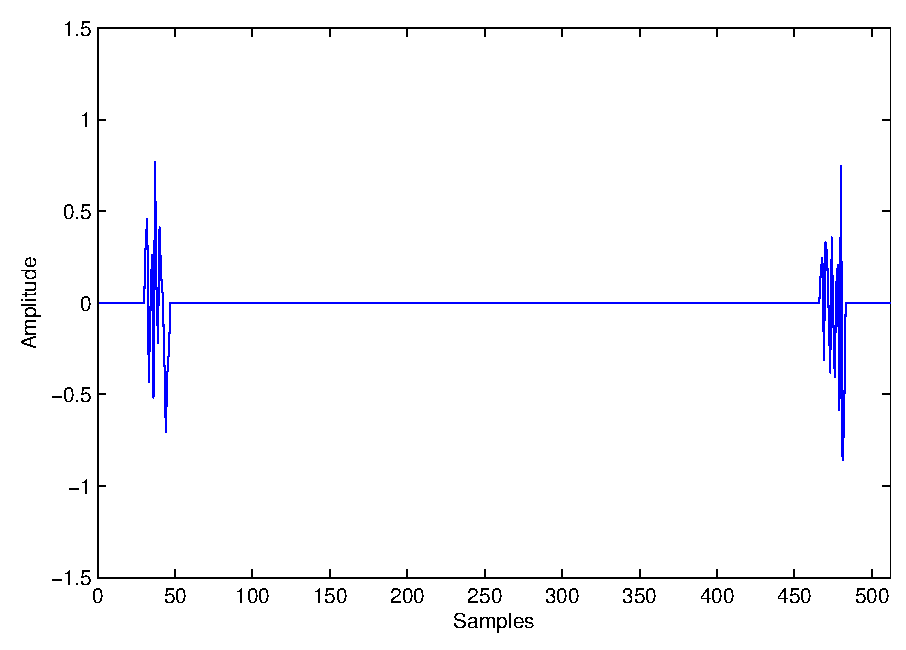
\includegraphics[width=11cm, height=8cm]{Figures/Chapter5/fig2b.eps}\\
\end{center}
\vspace{-1cm}
\caption{Acoustic echo path with $N=512$.}
\label{fig2}
\vspace{1.5cm}
\end{figure}

%%%%%%%%%%%%%%%%%%%%%%%%%%%%%%%%%%%%%%%%%%%%%%%%%%%%%%%%%%%%%%%%%%%%%

\vspace{-0.3cm}
\section{Fixed Sparsity}\label{sec:5.2}
\vspace{-0.5cm}
\noindent All simulations of this section were done with the echo paths represented in Fig. \ref{fig1} and Fig. \ref{fig2} with length $N=256$ and $N=512$ respectively. The spareness measure of the impulse response is given by $\xi_{12}(\textbf{w}_0)=\frac{N}{N-\sqrt{N}}\left(1-\frac{\|\textbf{w}_0\|_1}{\sqrt{N}\|\textbf{w}_0\|_2}\right)$ \cite{Duttweiler}. The sparseness of the impulse response has been confirmed to be 0.6131, equivalent to G168 recommendation for standard acoustic impulse response  \cite{Morgan}. For each experiment, the far-end signal was either corrupted by an additive white Gaussian noise (AWGN) or additive correlated Gaussian noise (ACGN). In all the experiments, the results were averaged over 200 independent trials and all parameters were selected by many trials to obtain the best performances.

 %%%%%%%%%%%%%%%%%%%%%%%%%%%%%%%%%%%%%%%%%%%%%%%%%%%%%%%%%%%%%%%%%%%%%
\vspace{-0.3cm}
\subsection{Additive White Gaussian Noise}\label{sec:5.2.1}

%%%%%%%%%%%%%%%%%%%%%%%%%%%%%%%%%%%%%%%%%%%%%%%%%%%
\vspace{-0.5cm}
\subsection{Filter length, $N=256$}\label{sec:5.2.1.1}
\vspace{-0.5cm}
\noindent In this experiment, the performance of the proposed algorithm is compared to those of the NLMS, PNLMS, IPNLMS, ZA-LMS, RZA-LMS and NNCLMS  algorithms in AWGN environment. The echo path is represented by the impulse response shown in Fig. \ref{fig1}. A zero mean white Gaussian sequence is used as the input signal (i.e., the far-end signal). The output of the echo path is corrupted by another zero mean sequence (i.e. the near-end signal), with a signal-to-noise ratio (SNR) of 30dB. For all the algorithms, simulations were done with the parameters given in Table \ref{table1}. Fig. \ref{fig3} shows that the NLMS, PNLMS and IPNLMS algorithms exhibit a slower convergence behavior than ZA-LMS algorithm with almost the same MSD estimate. The RZA-LMS algorithm converges faster than the previous algorithms with 1.5 dB lower MSD. The NNCLMS algorithm converges at the same rate with the ZA-LMS algorithm but achieves 1 dB lower MSD. However, the proposed algorithm converges at the same rate with the NNCLMS algorithm but gives 2 dB lower MSD. This will be on the account of some extra computations. However, the basic proportionate type adaptive filters displayed a slower convergence and poor tracking ability compared to the $l_1$-norm and $p$-norm  based sparse adaptive filters. This is because these algorithms are designed for relatively low order filter types.

%%%%%%%%%%%%%%%%%%%%%%%%%%%%%%%%%%%%%%%%%%%%%%%%%%%

\begin{table}[!htb]
\centering
\caption{Parameters used for the experiment in Section \ref{sec:5.2.1.1}.}
\vspace{0.5cm}
\begin{tabular}{|c|c|c|c|c|c|c|c|c|c|}
 \hline
    \multirow{2}{*}{Algorithms} & \multicolumn{9}{c|}{$N=256$, AWGN}\\
    \cline{2-10}
    & $\mu$ & $\rho$ & $\varepsilon$ & $\kappa$ & $\gamma$ &$\alpha$ &$\mu_{max}$& $\mu_{min}$ & $\delta$\\
    \hline
     Proposed  & ---  & --- & 10 & 0.0001 & 0.001& 0.97 & 0.005 & 0.0035 & --- \\ \hline
     NNCLMS  &0.005 & ---  & 10  & 0.0019 & --- & --- & ---  & --- & ---  \\ \hline
   RZA-LMS & 0.0056 &0.000018 & 10 & --- & ---  & --- & ---  & --- & --- \\ \hline
   ZA-LMS  & 0.005 & 0.00018 & --- & --- & --- & ---  & --- & --- & --- \\ \hline
   IPNLMS & 0.2 & --- & 0.6 & --- & --- & -0.75 & --- & --- & 0.000001 \\ \hline
   PNLMS & 0.2 & 0.02 & --- & --- & 0.01 & --- & --- & --- & 0.00001 \\ \hline
   NLMS & 0.2 & --- & --- & --- & --- & --- & --- & --- &  0.00001\\
   \hline
\end{tabular}
\label{table1}
\end{table}

%%%%%%%%%%%%%%%%%%%%%%%%%%%%%%%%%%%%%%%%%%%%%%%%%%%

\begin{figure}[!htb]
\begin{center}
\vspace{1cm}
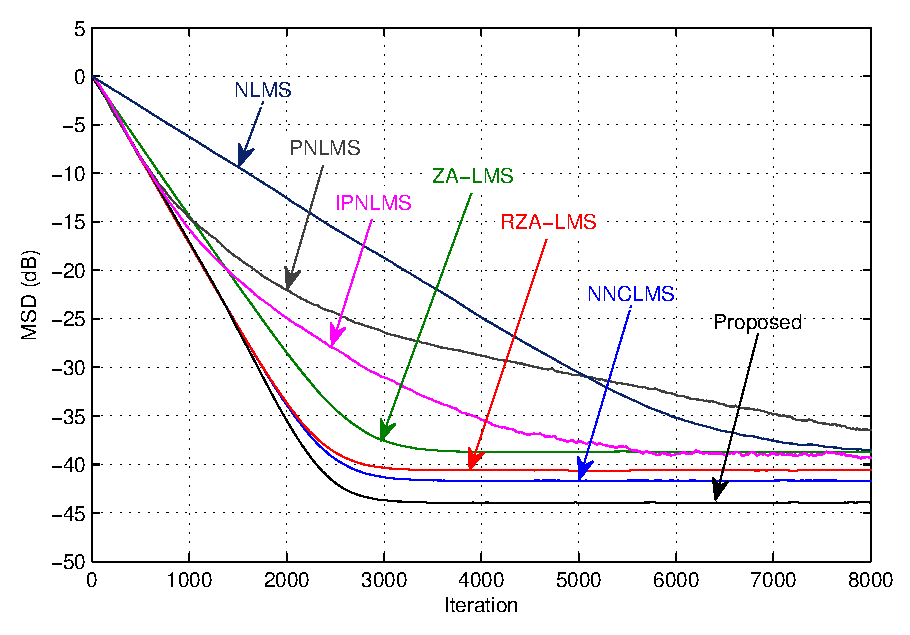
\includegraphics[width=14.25cm, height=11cm]{Figures/Chapter5/fig3a.eps}\\
\end{center}
\vspace{-1cm}
\caption{Ensemble learning curves of all algorithms in AWGN, SNR=30 dB and $N=256$.}
\label{fig3}
\vspace{1.5cm}
\end{figure}

%%%%%%%%%%%%%%%%%%%%%%%%%%%%%%%%%%%%%%%%%%%%%%%%%%%

\vspace{-0.3cm}
\subsection{Filter length, $N=512$}\label{sec:5.2.1.2}
\vspace{-0.5cm}
\noindent Due to the excessive length of the echo path, higher order adaptive filters are readily required for echo cancellation application. This affects the performance many of the available adaptive filters. To test the performance of the proposed algorithm due to long acoustic impulse response, we used a filter order of $N=512$ to simulate the acoustic path represented in Fig. \ref{fig2} with length $N=512$. The standard sparseness degree (0.6131) is also maintained. The experiment was implemented with the same input signal and noise of the experiment in Section \ref{sec:5.2.1}. Simulations were done with the parameters given in Table \ref{table2}. From the table it can be observed that the step-size parameters of the proposed algorithm decreased as the filter length is increased as expected. We notice from Fig. \ref{fig4} that, even though the filter length is increased,  the proposed algorithm performance remains superior compared to the other algorithms.


%%%%%%%%%%%%%%%%%%%%%%%%%%%%%%%%%%%%%%%%%%%%%%%%%%%%%%%%%%%%%%%%%%%%%%%%%%%%%%%%%%%%%%%%
\begin{figure}[!htb]
\begin{center}
\vspace{1cm}
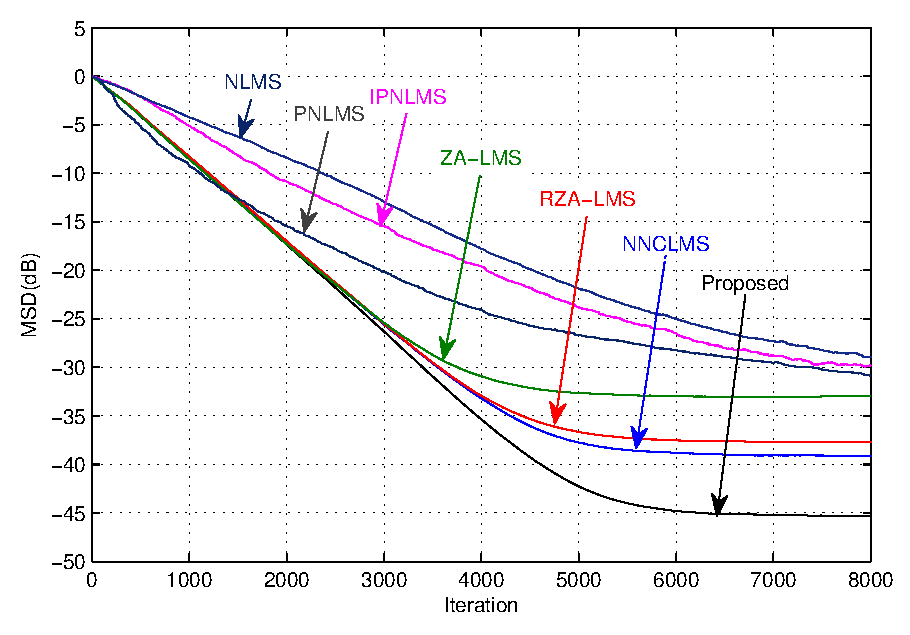
\includegraphics[width=14.25cm, height=11cm]{Figures/Chapter5/fig4.eps}\\
\end{center}
\vspace{-1cm}
\caption{Ensemble learning curves of all algorithms in AWGN, SNR=30 dB and $N=512$.}
\label{fig4}
\vspace{1.5cm}
\end{figure}


%%%%%%%%%%%%%%%%%%%%%%%%%%%%%%%%%%%%%%%%%%%%%%%%%%%%%%%%%%%%%%%%%%%%%%%%%%%%%%%%%%%%%%%%%%%
\begin{table}[!htb]
\centering
\caption{Parameters used for the experiment in Section \ref{sec:5.2.1.2}.}
\vspace{0.5cm}
\begin{tabular}{|c|c|c|c|c|c|c|c|c|c|}
 \hline
    \multirow{2}{*}{Algorithms} & \multicolumn{9}{c|}{$N=512$, AWGN}\\
    \cline{2-10}
    & $\mu$ & $\rho$ & $\varepsilon$ & $\kappa$ & $\gamma$ &$\alpha$ &$\mu_{max}$& $\mu_{min}$ & $\delta$\\
    \hline
     Proposed  & --- & --- & 10 & 0.002 & 0.002& 0.91 & 0.0025 & 0.0015 & ---  \\ \hline
     NNCLMS  & 0.0025 & ---  & 10  & 0.000016 & --- & --- & --- & --- & ---  \\ \hline
   RZA-LMS & 0.0025 & 0.000018 & 10 & --- & --- & --- & --- & --- & ---  \\ \hline
   ZA-LMS  & 0.0025 & 0.00011 & --- & --- & --- & --- & --- & --- & ---  \\ \hline
   IPNLMS & 0.32 & --- & 0.6 & --- & --- & -0.75 & --- & --- & 0.000001 \\ \hline
   PNLMS & 0.3 & 0.097 & --- & --- & 0.01 & --- & --- & --- & 0.000001 \\ \hline
   NLMS & 0.3 & --- & --- & --- & --- & --- & --- & --- &  0.000001\\ \hline
\end{tabular}
\label{table2}
 \end{table}
%%%%%%%%%%%%%%%%%%%%%%%%%%%%%%%%%%%%%%%%%%%%%%%%%%%%%%%%%%%%%%%%%%%%%%%%%%%%%%%%%%%%%%%%%%%

\vspace{-0.3cm}
\subsection{Additive Correlated Gaussian Noise}\label{sec:5.2.2}
\vspace{-0.5cm}
\noindent In order to see how the proposed algorithm is robust to the noise type, an ACGN is added to the input signal. The ACGN process is created using the first-order autoregressive (AR(1)) model defined as:
%%%%%%%%%%%%%%%%%%%%%%%%%%%%%%%%%%%%%%%%%%%%%%%%%%%%%%%%

\vspace{-1cm}
\begin{equation}
\eta(n)=\wp\eta(n-1)+v(n),\label{eq_1q}
\end{equation}
\vspace{-1cm}

%%%%%%%%%%%%%%%%%%%%%%%%%%%%%%%%%%%%%%%%%%%%%%%%%%%%%%%%
\noindent where $\wp$ is a correlation parameter and $v(n)$ is a white Gaussian process with zero mean and a variance that provides a 30 dB SNR.
%%%%%%%%%%%%%%%%%%%%%%%%%%%%%%%%%%%%%%%%%%%%%%%%%%%%%%%%%%%%%%%%%%%%%%
\vspace{-0.3cm}
\subsection{Low Correlated Gaussian Noise}\label{sec:5.2.2.1}
\vspace{-0.5cm}
\noindent In this experiment, we study the effect of low correlated Gaussian noise environment on the performance of the proposed algorithm. The low correlated Gaussian noise process was obtained from the AR(1) model generated in (\ref{eq_1q}) by setting the correlation parameter to be $\wp=0.45$ while maintaining the SNR value. In this case, we used a filter order of $N=256$, which is equivalent to the length of the echo path depicted in Fig. \ref{fig1}. All the algorithms were implemented using the parameters given in Table \ref{table3}. From Fig. \ref{fig5}, we observe that the proposed algorithm still provides the best performance with 1.5 dB lower MSD than the best of other algorithms. In the other hand, the proposed algorithm is faster than the best performer among the other algorithms by almost 200 iterations. This is by the virtue of the variable step-size which shows the ability of the proposed algorithm in suppressing correlated noise.

%%%%%%%%%%%%%%%%%%%%%%%%%%%%%%%%%%%%%%%%%%%%%%%%%%%%%%%%%%%%%%%%%%%%%%%
\begin{figure}[!htb]
\begin{center}
\vspace{1cm}
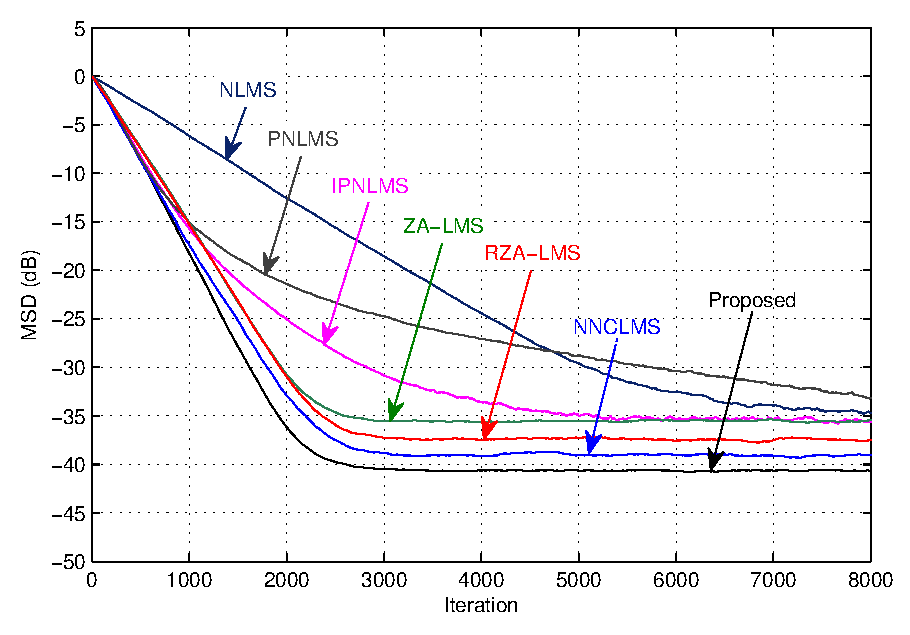
\includegraphics[width=14.25cm, height=11cm]{Figures/Chapter5/fig5.eps}\\
\end{center}
\vspace{-1cm}
\caption{Ensemble learning curves of all algorithms in low correlated ACGN, SNR=30 dB and $N=256$.}
\label{fig5}
\vspace{1.5cm}
\end{figure}

%%%%%%%%%%%%%%%%%%%%%%%%%%%%%%%%%%%%%%%%%%%%%%%%%%%%%%%%%%%%%%%%%%%%%%%
\begin{table}[!htb]
\centering
\caption{Parameters used for the experiment in Section \ref{sec:5.2.2.1}.}
\vspace{0.5cm}
\begin{tabular}{|c|c|c|c|c|c|c|c|c|c|}
 \hline
    \multirow{2}{*}{Algorithms} & \multicolumn{9}{c|}{$N=256$, ACGN}\\
    \cline{2-10}
    & $\mu$ & $\rho$ & $\varepsilon$ & $\kappa$ & $\gamma$ &$\alpha$ & $\mu_{max}$ & $\mu_{min}$ & $\delta$ \\
    \hline
     Proposed  & --- & --- & 10 & 0.001 & 0.001& 0.97 & 0.0056 & 0.0045 & --- \\ \hline
     NNCLMS  &0.0035 & ---  & 10  & 0.0019 & --- & --- & --- & --- & ---  \\ \hline
   RZA-LMS & 0.0045 &0.000018 & 10 & --- & --- & --- & --- & --- & --- \\ \hline
   ZA-LMS  & 0.005 & 0.000018 & --- & --- & --- & --- & --- & --- & ---  \\ \hline
   IPNLMS & 0.2 & --- & 0.6 & --- & --- & -0.75 & --- & --- & 0.000001 \\ \hline
   PNLMS & 0.2 & 0.02 & --- & --- & 0.01 & --- & --- & --- & 0.00001  \\ \hline
   NLMS & 0.2 & --- & --- & --- & --- & --- & --- & --- &  0.00001  \\ \hline
\end{tabular}
\label{table3}
 \end{table}

%%%%%%%%%%%%%%%%%%%%%%%%%%%%%%%%%%%%%%%%%%%%%%%%%%%%%

\vspace{-0.3cm}
\subsection{Highly Correlated Gaussian Noise}\label{sec:5.2.2.2}
\vspace{-0.5cm}
\noindent In this experiment, we investigate the performance of the proposed algorithm in relatively high correlated noise environment. The input signal is assumed to be corrupted by ACGN process generated by the AR(1) model created in (\ref{eq_1q}), with the correlation parameter set to $\wp=0.7$ ( i.e., relatively high correlated Gaussian noise) with the same SNR value. The experiment was done with the parameters provided in Table \ref{table3}. Fig. \ref{fig6} shows that with the relatively high ACGN, the NLMS, PNLMS and IPNLMS algorithms have shown poor performances in terms of MSD and convergence rate values. However, the proposed algorithm provides the best MSD estimate among all algorithms (2 dB, 4 dB and 7 dB lower MSD than the NNCLMS, RZA-LMS and ZA-LMS algorithms, respectively). This shows that, despite the high MSD estimate provided by all the algorithms in a relatively high correlated noise environment, the proposed algorithm outperforms all other algorithms in terms of the MSD estimate.

%%%%%%%%%%%%%%%%%%%%%%%%%%%%%%%%%%%%%%%%%%%%%%%%%%%%%

\begin{figure}[!htb]
\begin{center}
\vspace{1cm}
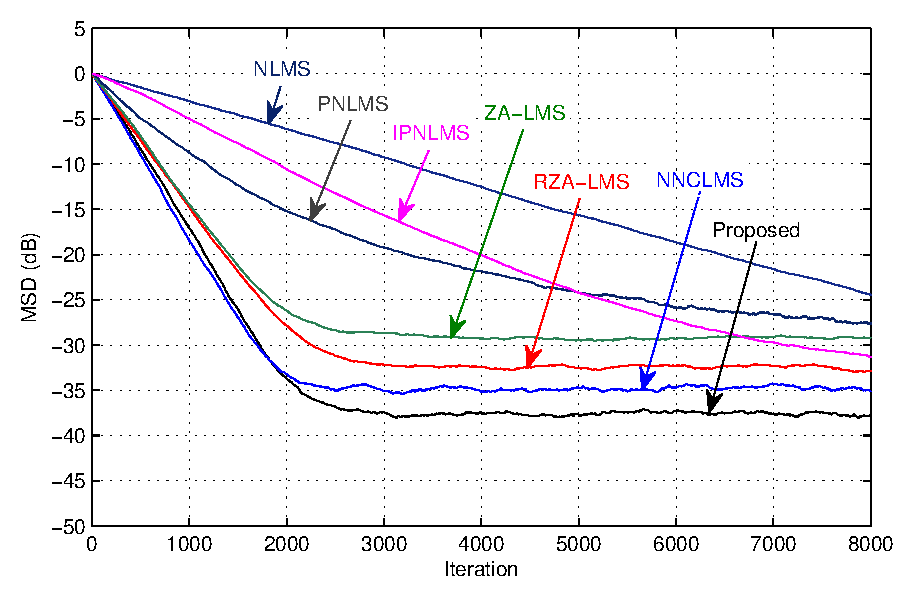
\includegraphics[width=14.25cm, height=11cm]{Figures/Chapter5/fig6.eps}\\
\end{center}
\vspace{-1cm}
\caption{Ensemble learning curves of all the algorithms in highly correlated ACGN, SNR=30 dB and $N=256$.}
\label{fig6}
\vspace{1.5cm}
\end{figure}
%%%%%%%%%%%%%%%%%%%%%%%%%%%%%%%%%%%%%%%

\begin{figure}[!htb]
\begin{center}
\vspace{1cm}
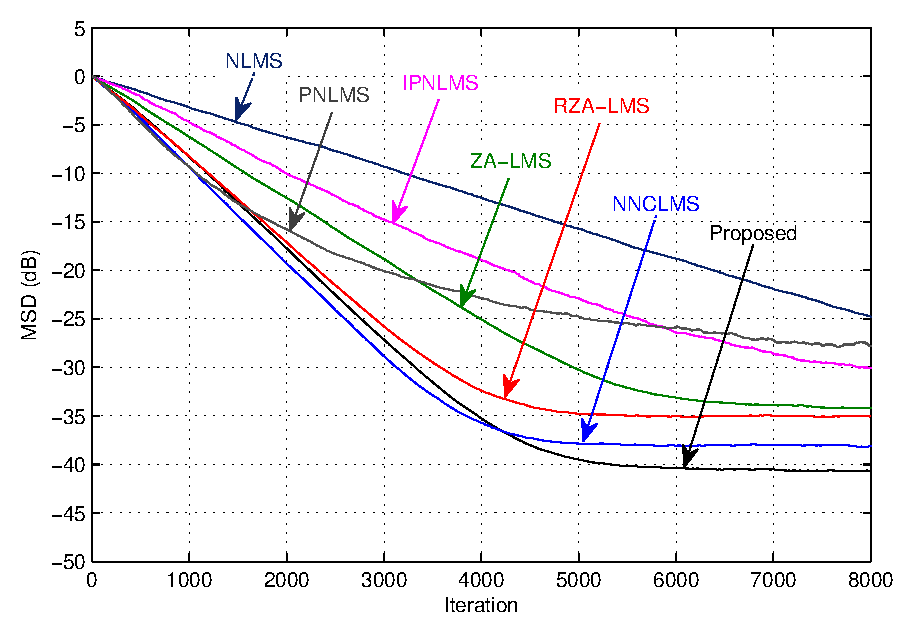
\includegraphics[width=14.25cm, height=11cm]{Figures/Chapter5/fig7.eps}\\
\end{center}
\vspace{-1cm}
\caption{MSD curves of all algorithms in ACGN, $N=512$.}
\label{fig7}
\vspace{1.5cm}
\end{figure}

%%%%%%%%%%%%%%%%%%%%%%%%%%%%%%%%%%%%%%%%%%%%%%%%%%%%%
\vspace{-0.5cm}
\par
\noindent Since the performance of all algorithms degrade a little in high correlated noise environments, we will proceed to investigate the performance of the proposed algorithm in only low correlated noise environments using a higher order filter. Therefore, in this experiment, the performance of the proposed algorithm is tested due to excessive length of the echo path in a low correlated Gaussian noise environment by repeating the experiment in Section \ref{sec:5.2.2.1}, but with a filter length $N=512$ and the echo path represented in Fig. \ref{fig2}. The correlated signal used in this case, which is usually encountered in acoustic echo cancellation problems is created exactly as in the same Section \ref{sec:5.2.2.1}. The parameters used for the simulations are provided in Table \ref{table4}. It can be seen from  Fig. \ref{fig7} that the NLMS, PNLMS and IPNLMS algorithms fail to reach the steady-state MSD within the time extent shown. However, even though all algorithms display slow convergence behavior, the proposed algorithm is a little bit faster than the others. In terms of MSD estimate, the proposed algorithm gives an improvement of 3 dB, 6 dB and 7 dB compared to NNCLMS, RZA-LMS and ZA-LMS algorithms, respectively. Hence, despite the length of the echo path and the effect of the correlation parameter, the proposed algorithm performs robustly and better than the rest of algorithms both in convergence rate and MSD estimate. The NLMS algorithm is clearly seen to provide poor performance among others. The proportionate updating based optimization approach utilized by PNLMS and IPNLMS algorithms is observed to be inefficient for this experimental settings and, therefore, they provide unsatisfactory performances compared to NNCLMS, RZA-LMS and ZA-LMS algorithms.

%%%%%%%%%%%%%%%%%%%%%%%%%%%%%%%%%%%%%%%%%%%%%%%%%%%%%%%%%%%%%%%%%%%%%%%%%

\begin{table}[!htb]
\centering
\caption{Parameters for the experiment in Section \ref{sec:5.2.2.2}.}
\vspace{0.5cm}
\begin{tabular}{|c|c|c|c|c|c|c|c|c|c|}
 \hline
    \multirow{2}{*}{Algorithms} & \multicolumn{9}{c|}{$N=512$, ACGN}\\
    \cline{2-10}
    & $\mu$ & $\rho$ & $\varepsilon$ & $\kappa$ & $\gamma$ &$\alpha$ &$\mu_{max}$& $\mu_{min}$ & $\delta$\\
    \hline
     Proposed  & --- & --- & 10 & 0.00001 & 0.0001& 0.91 & 0.0025 & 0.0015 & --- \\ \hline
     NNCLMS  &0.0027 & --- & 10  & 0.0017 & --- & --- & --- & --- & ---  \\ \hline
   RZA-LMS & 0.0027 &0.000018 & 10 & --- & --- & --- & ---  & --- & --- \\ \hline
   ZA-LMS  & 0.0027 & 0.00011 & --- & --- & --- & --- & --- & --- & --- \\ \hline
   IPNLMS & 0.3 & --- & 0.5 & --- & --- & -0.75 & --- & --- & 0.000001 \\ \hline
   PNLMS & 0.3 & 0.01 & --- & --- & 0.01 & --- & --- & --- & 0.000001  \\ \hline
   NLMS & 0.38 & --- & --- & --- & --- & --- & --- & --- &  0.000001  \\ \hline
\end{tabular}
\label{table4}
 \end{table}

%%%%%%%%%%%%%%%%%%%%%%%%%%%%%%%%%%%%%%%%%%%%%%%%%%%%%%%%%%%%%%%%%%%%%%%%%
Up to now, it has been noticed that the performances of the NLMS, PNLMS and IPNLMS algorithms are very poor in terms of MSD and convergence rate. Hence, these algorithms will be excluded from the experiments that appear in the rest of this chapter.


\vspace{-0.3cm}
\section{Performance of the Proposed Algorithm under Different Sparsity Ratios}\label{sec:5.3}
\vspace{-0.5cm}
\noindent In this section, two experiments are performed to find out the effect of the sparsity on the performance of the proposed  by changing the sparsity ratio of the unknown system. One experiment is performed in AWGN and the other one is designed for ACGN environment. For ease of implementation, a filter order $N=256$ taps was used in all the experiments. Because of the poor performances demonstrated by the NLMS, PNLMS and IPNLM algorithms in all the previous experiments under similar experimental set up, we would in this section  focus on testing the performance of the proposed algorithm and compare with only those of the $l_1$-norm and $p$-norm based sparse algorithms (i.e., ZA-LMS, RZA-LMS and NNCLMS algorithms).

%%%%%%%%%%%%%%%%%%%%%%%%%%%%%%%%%%%%%%%%%%%%%%%%%%%%%%%%%%%%%%%%%%%%%%%%%
\vspace{-0.3cm}
\subsection{Additive White Gaussian Noise}\label{sec:5.3.1}
\vspace{-0.5cm}
\noindent This experiment is performed to test and compare the convergence and tracking ability of the proposed algorithm compare with those of the NNCLMS, RZA-LMS and ZA-LMS algorithms in identifying unknown systems with different sparsity conditions. The used acoustic echo path is represented in Fig. \ref{fig1}. The SNR is assumed to be 30 dB. In this scenario, the same system is made to be 75\%, 50\%, and 25\% sparse (i.e. at 75\% sparsity, 192 taps are made inactive while the rest are made active, etc.). The metric used for measuring the sparseness level is the same as the one used in Section \ref{sec:5.2}. Simulations were done with parameters given in Table \ref{table1}. Figs. \ref{fig8}, \ref{fig9} and \ref{fig10} show the results of the MSD between the echo path coefficients and the adaptive filter coefficients at 75\%, 50\%, and 25\% sparsity ratio, respectively. Table \ref{table5} shows a summary of the obtained results. It can be observed that, at 75\% sparse system, the proposed algorithm converges slower than the rest by 200 iterations but achieves a better MSD estimate of 5 dB, 9 dB and 11 dB than the NNCLMS, RZA-LMS and ZA-LMS algorithms, respectively. At 50\% sparsity ratio, all algorithms have the same convergence rate but the proposed algorithm still outperforms the rest in terms of MSD estimate. But when the unknown system is 25\% sparse, both the proposed algorithm and NNCLMS algorithm converge at the same rate but slower than the RZA-LMS and ZA-LMS algorithms with lower MSD of the proposed algorithm. The convergence behavior of RZA-LMS and ZA-LMS algorithms with such high MSD is due to their lack of adjustable factors that can adapt the norm constraint during the filtering process. In addition, we notice that the proposed algorithm shows a similar convergence in all the three sparsity ratios and shows an outstanding performance in MSD estimate compared to other algorithms in every sparsity condition of the unknown system. This experiment shows that the convergence rate and tracking ability of the proposed algorithm is less sensitive to the sparseness degree of the acoustic impulse response and less affected in terms of MSD estimate.

%%%%%%%%%%%%%%%%%%%%%%%%%%%%%%%%%%%%%%%%%%%%%%%%%%%%%%%%%%%%%%%%%%%%
\begin{figure}[!htb]
\begin{center}
\vspace{1cm}
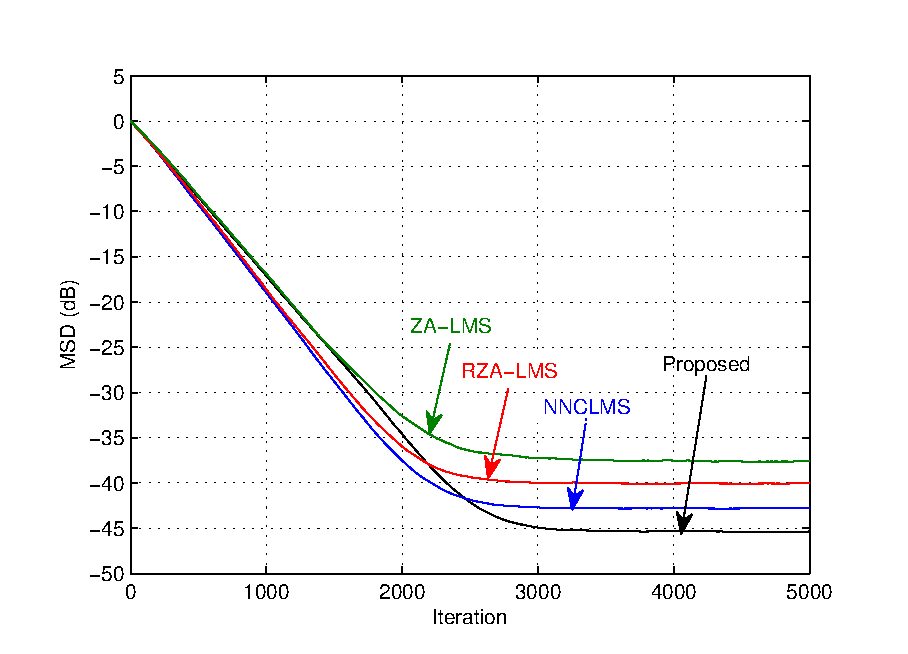
\includegraphics[width=16.5cm, height=12cm]{Figures/Chapter5/fig10.eps}\\
\end{center}
\vspace{-1cm}
\caption{Tracking and steady-state behaviors of a 256 taps adaptive filters with 75\% sparsity ratio in AWGN.}
\label{fig8}
\vspace{1.5cm}
\end{figure}

%%%%%%%%%%%%%%%%%%%%%%%%%%%%%%%%%%%%%%%%%%%%%%%%%%%%%%%%%%%%%%%%%%%%%%%%
\begin{figure}[!htb]
\begin{center}
\vspace{1cm}
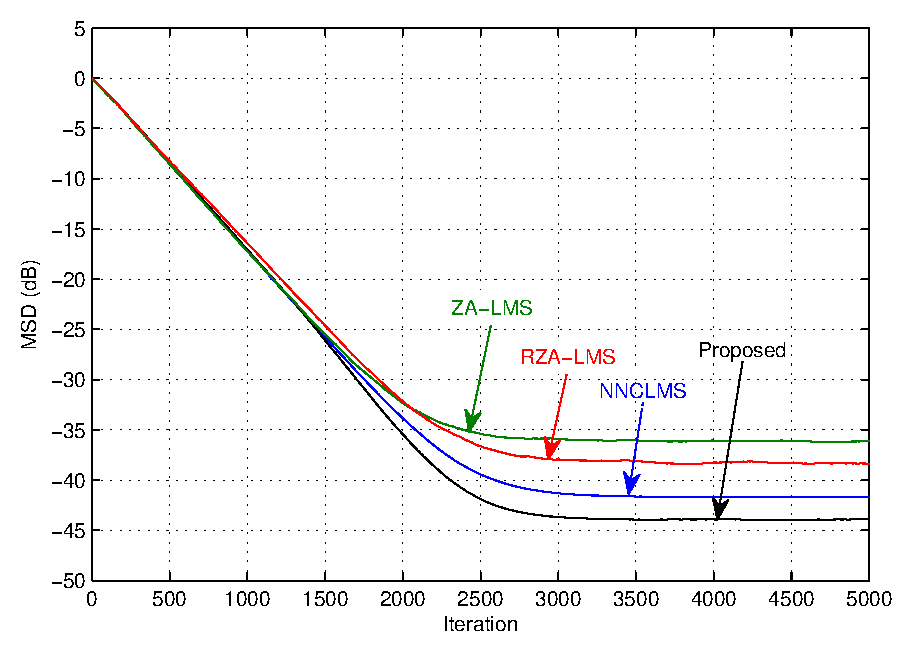
\includegraphics[width=14.25cm, height=11cm]{Figures/Chapter5/fig9.eps}\\
\end{center}
\vspace{-1cm}
\caption{Tracking and steady-state behaviors of a 256 taps adaptive filters with 50\% sparsity ratio in AWGN.}
\label{fig9}
\vspace{1.5cm}
\end{figure}
%%%%%%%%%%%%%%%%%%%%%%%%%%%%%%%%%%%%%%%%%%%%%%%%%%%%%%%%%%%%%%%%%%%%%%%
\begin{figure}[!htb]
\begin{center}
\vspace{1cm}
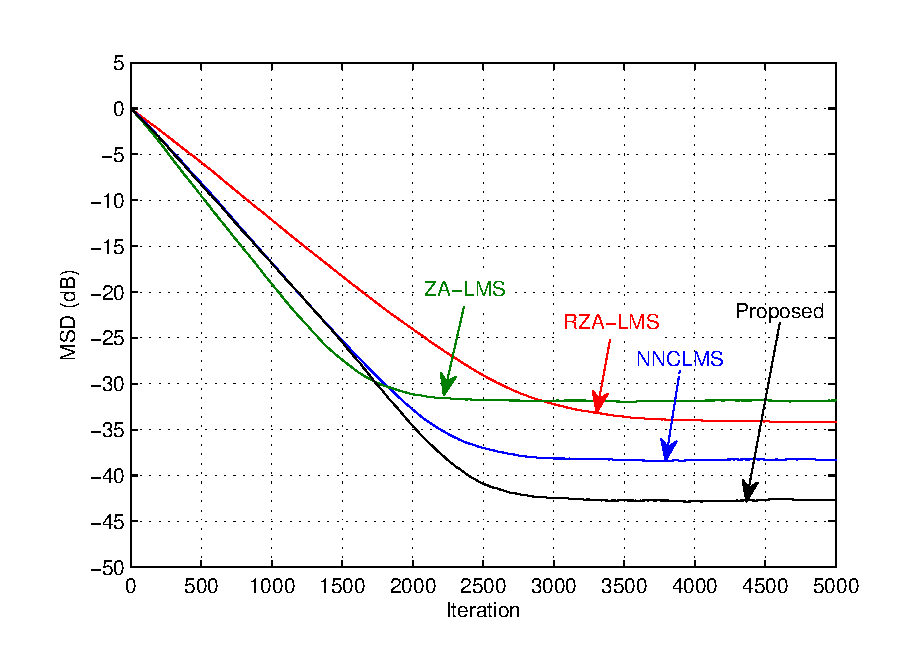
\includegraphics[width=16cm, height=12cm]{Figures/Chapter5/fig8.eps}\\
\end{center}
\vspace{-1cm}
\caption{Tracking and steady-state behaviors of a 256 taps adaptive filters with 25\% sparsity ratio in AWGN.}
\label{fig10}
\vspace{1.5cm}
\end{figure}

%%%%%%%%%%%%%%%%%%%%%%%%%%%%%%%%%%%%%%%%%%%%%%%%%%%%%%%%%%%%%%%%%%%%%%%%
 \begin{table}[!htb]
\centering
\caption{Results for experiment in Section \ref{sec:5.3.1}.}
\vspace{0.5cm}
\begin{tabular}{|c|c|c|c|c|c|c|}
 \hline
 \multirow{2}{*}{Algorithm} & \multicolumn{2}{c|}{75\% sparse} & \multicolumn{2}{c|}{50\% sparse} & \multicolumn{2}{c|}{25\% sparse} \\
 \cline{2-7}
  & Convergence  & MSD(dB) & Convergence & MSD(dB) &Convergence & MSD(dB)\\ \hline
  Proposed & 3000 & $-45.1$ & 3000 & $-44$ & 3000  & $-43$ \\ \hline
  NNCLMS  & 2800 & $-42.5$ & 3000 & $-42$ & 3000  & $-38$  \\ \hline
  RZA-LMS &2800  & $-40$ & 3000 & $-40.5$ & 3250 & $-34$   \\ \hline
  ZA-LMS & 2800  & $-37.5$ &3000 & $-36$ & 2250 & $-32$ \\ \hline
  \end{tabular}
  \label{table5}
  \end{table}

%%%%%%%%%%%%%%%%%%%%%%%%%%%%%%%%%%%%%%%%%%%%%%%%%%%%%%%%%%%%%%%%%%%%%%
\vspace{-0.3cm}
\subsection{Additive Correlated Gaussian Noise}\label{sec:5.3.2}
\vspace{-0.5cm}
\noindent The same experiment of Section \ref{sec:5.3.2} is repeated with only replacing the AWGN by an ACGN process. The ACGN process is created as in  Section \ref{sec:5.2.2.1} and with the echo path depicted in Fig. \ref{fig1}. Simulations were done with the parameters provided in Table \ref{table2}. The average MSD estimate between the adaptive filter coefficients and the unknown system coefficients of all algorithms are shown in Figs. \ref{fig11}, \ref{fig12} and \ref{fig13} at 75\%, 50\%, and 25\% sparsity ratios, respectively. A summary of the obtained results is provided in Table \ref{table6}. We notice that, at 75\% sparsity ratio, the proposed algorithm converges faster than the rest algorithms by almost 100 iterations and achieves a better MSD estimate (2.1 dB, 3.1 dB, and 3.6 dB) than NNCLMS, RZA-LMS and ZA-LMS, respectively. This shows the ability of the proposed algorithm in suppressing a correlated noise in sparse system. When the unknown system is set to 50\% sparsity ratio, we still notice almost similar behavior except that the RZA-LMS shows a slower convergence by about 500 iterations and achieves a little higher MSD of almost 0.5 dB than when the unknown system is 75\% sparse. But when the unknown system is at 25\% sparsity ratio, we notice deterioration in the performance of the NNCLMS, RZA-LMS and ZA-LMS algorithms, with the ZA-LMS algorithm worse among all of them. However, the proposed algorithm still retains its superior performance. This is because the proposed algorithm achieves a lower MSD improvement of almost 2.5 dB, 5 dB and 9 dB compared to NNCLMS, RZA-LMS and ZA-LMS, respectively.

\vspace{-0.5cm}
\par
\noindent In this experiment, it can be noted that the convergence behavior of the proposed algorithm remains the same in all three sparsity conditions of the unknown system. The proposed algorithm also gives a better MSD estimates in all given sparsity settings. This is due to the ability of the $p$-norm constraint to efficiently exploit the unknown system's sparsity and the virtue of the variable step-size to track the changes of the unknown system. Even though, the ACGN process causes a little higher MSD estimate, the proposed algorithm has been observed to be more robust among the others in correlated noise environments.
We also notice from the result that, unlike when an AWGN is used, all algorithms achieve higher MSD estimate in correlated environment. However, despite this challenge we still observed that the proposed algorithm shows the same convergence rate across every sparsity condition of the system and simultaneously outperform all algorithms in terms of MSD estimates.

%%%%%%%%%%%%%%%%%%%%%%%%%%%%%%%%%%%%%%%%%%%%%%%%%%%%%%%%%%%%%%%%%%%%%%


%%%%%%%%%%%%%%%%%%%%%%%%%%%%%%%%%%%%%%%%%%%%%%%%%%%%%%%%%%%%%%%%%%%%%%%%%%%%%%%%

\begin{figure}[!htb]
\begin{center}
\vspace{1cm}
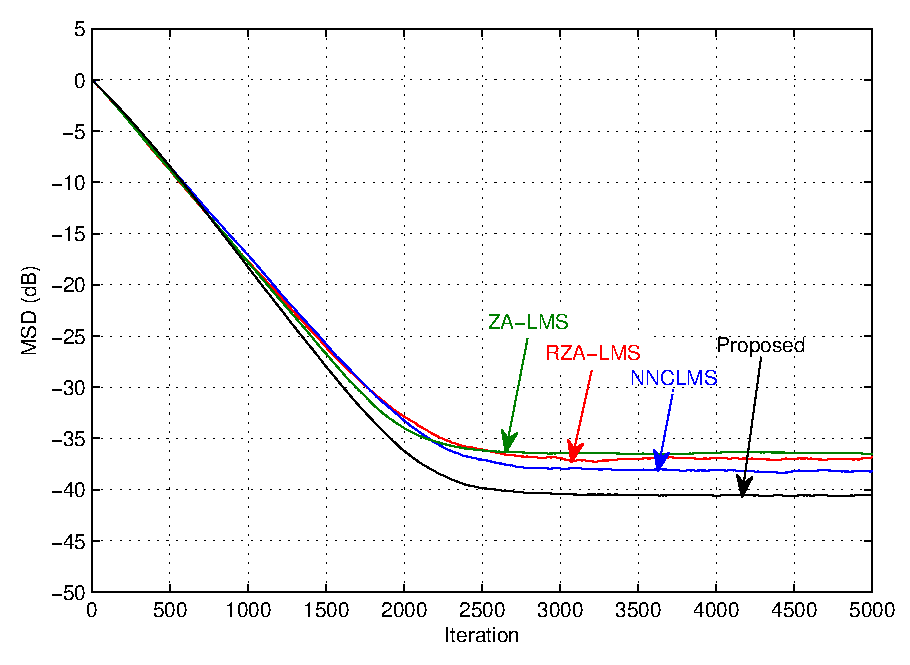
\includegraphics[width=14.25cm, height=11cm]{Figures/Chapter5/fig13.eps}\\
\end{center}
\vspace{-1cm}
\caption{Tracking and steady-state behaviors of a 256 taps adaptive filters with 75\% sparsity ratio in ACGN.}
\label{fig11}
\vspace{1.5cm}
\end{figure}


%%%%%%%%%%%%%%%%%%%%%%%%%%%%%%%%%%%%%%%%%%%%%%%%%%%%%%%%%%%%%%%
\begin{figure}[!htb]
\begin{center}
\vspace{1cm}
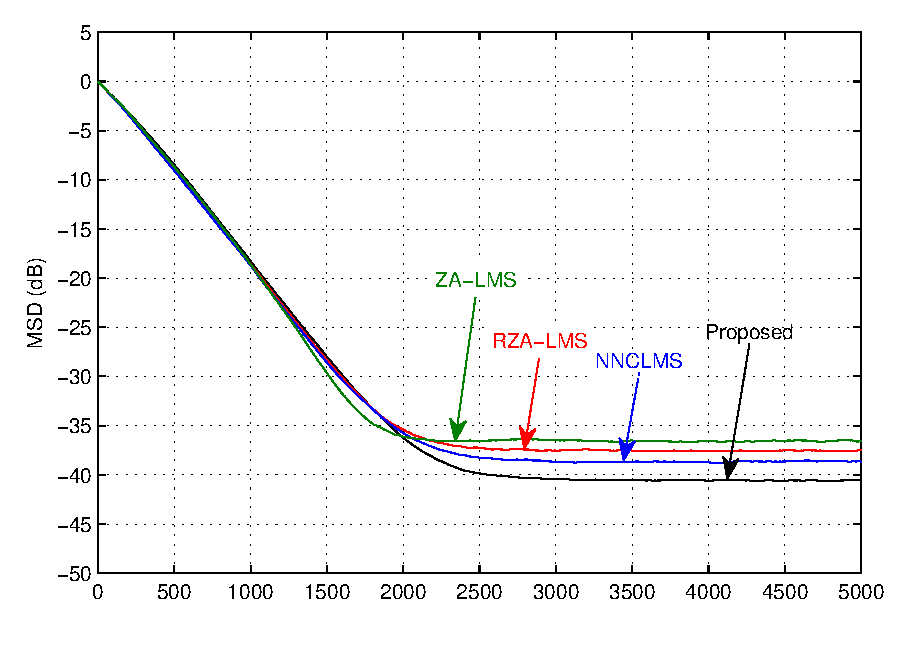
\includegraphics[width=15cm, height=11.2cm]{Figures/Chapter5/fig12.eps}\\
\end{center}
\vspace{-1cm}
\caption{Tracking and steady-state behaviors of a 256 taps adaptive filters with 50\% sparsity ratio in ACGN.}
\label{fig12}
\vspace{1.5cm}
\end{figure}

%%%%%%%%%%%%%%%%%%%%%%%%%%%%%%%%%%%%%%%%%%%%%%%%%%%%%%%%%%%%%%%%%%
\begin{figure}[!htb]
\begin{center}
\vspace{1cm}
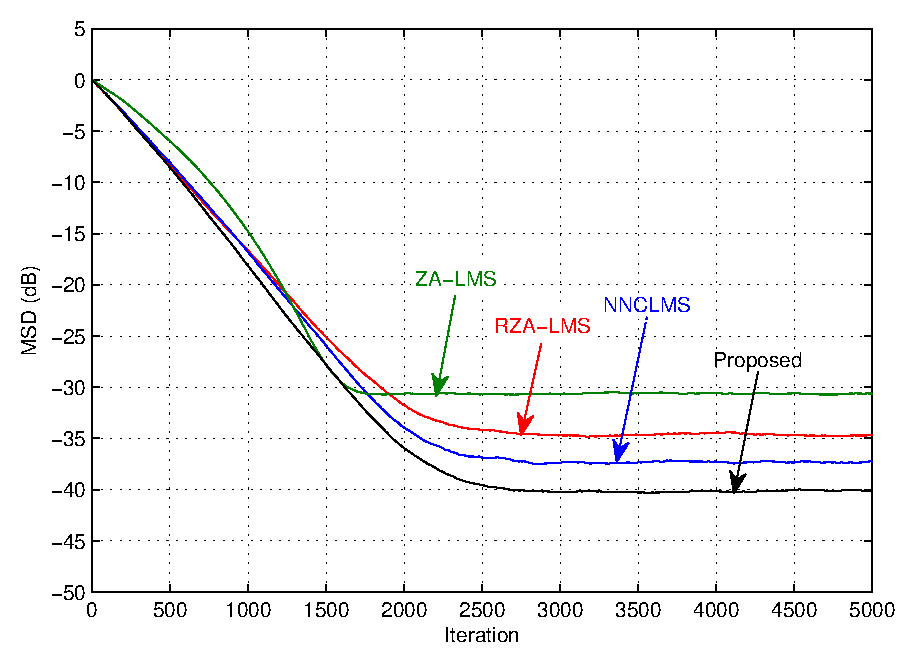
\includegraphics[width=14.5cm, height=11.5cm]{Figures/Chapter5/fig11.eps}\\
\end{center}
\vspace{-1cm}
\caption{Tracking and steady-state behaviors of a 256 taps adaptive filters with 25\% sparsity ratio in ACGN.}
\label{fig13}
\vspace{1.5cm}
\end{figure}


%%%%%%%%%%%%%%%%%%%%%%%%%%%%%%%%%%%%%%%%%%%%%%%%%%%%%%%%%%%%%%%%%%%%%%%%%%%%%%%%

\begin{table}[!htb]
\centering
\caption{Results for experiment in Section \ref{sec:5.3.2}.}
\vspace{0.5cm}
\begin{tabular}{|c|c|c|c|c|c|c|}
 \hline

  \multirow{2}{*}{Algorithm} & \multicolumn{2}{c|}{75\% sparse} & \multicolumn{2}{c|}{50\% sparse} & \multicolumn{2}{c|}{25\% sparse} \\
  \cline{2-7}
    & Convergence & MSD(dB) & Convergence  & MSD(dB) &Convergence& MSD(dB)\\ \hline
    Proposed & 2500 & $-40.1$ & 2500 & $-40.1$ & 2500  & $-40$ \\ \hline
    NNCLMS  & 2600 & $-38$ & 2500 & $-38$ & 2500  & $-37.5$  \\ \hline
   RZA-LMS & 2600 & $-37$ & 2500 & $-37$ & 2500 & $-35$   \\ \hline
   ZA-LMS & 2600 & $-36.5$ &  2000 & $-36$ & 1700 & $-31$ \\ \hline
  \end{tabular}
  \label{table6}
  \end{table}

%%%%%%%%%%%%%%%%%%%%%%%%%%%%%%%%%%%%%%%%%%%%%%%%%%%%%%%%%%%%%%%%%%%%%%%%%%%%%%%%

